\renewcommand{\thechapter}{2}
\chapter{The EXO-200 Detector}

This chapter will describe the physical apparatus of the EXO-200 detector.  Section~\ref{sec:DetectorOverview} will give a broad overview of the detector.  Section~\ref{sec:DetectorBackgrounds} will identify the dominant backgrounds for $\beta\beta 0\nu$ decay, and sections~\ref{sec:DetectorPassiveBackgroundRejection} and \ref{sec:DetectorActiveBackgroundRejection} will describe methods used to mitigate these backgrounds.  The pulse and waveform readout subsystems are described in section~\ref{sec:DetectorReadout}, where discussion of the scintillation readout will be particularly important for subsequent chapters.  We conclude with a description of the calibration systems in section~\ref{sec:DetectorCalibration}.  Throughout, the reader is referred to the detailed description in~\cite{detectorPartI} for more information.

\section{Overview of the EXO-200 Detector}\label{sec:DetectorOverview}

The EXO-200 detector is a cryogenic experiment containing $175$ kg of liquid xenon enriched to $80.6\%$ in $^{136}$Xe.  Of those $175$ kg of liquid xenon, $110$ kg are contained within the ``active'' volume where the detector is fully sensitive to deposited energy from $\beta\beta$ decay,~\cite{detectorPartI} and $94.7$ kg are contained within the fiducial volume where we believe the detector's response is well-understood.  Only fiducial xenon will be used in the search for $\beta\beta 0\nu$ decay; this means there are $3.39 \cdot 10^{26}$ atoms $^{136}$Xe which will be used for setting half-life limits.~\cite{NewEXObb0nPaper_2014}

\begin{figure}
\begin{center}
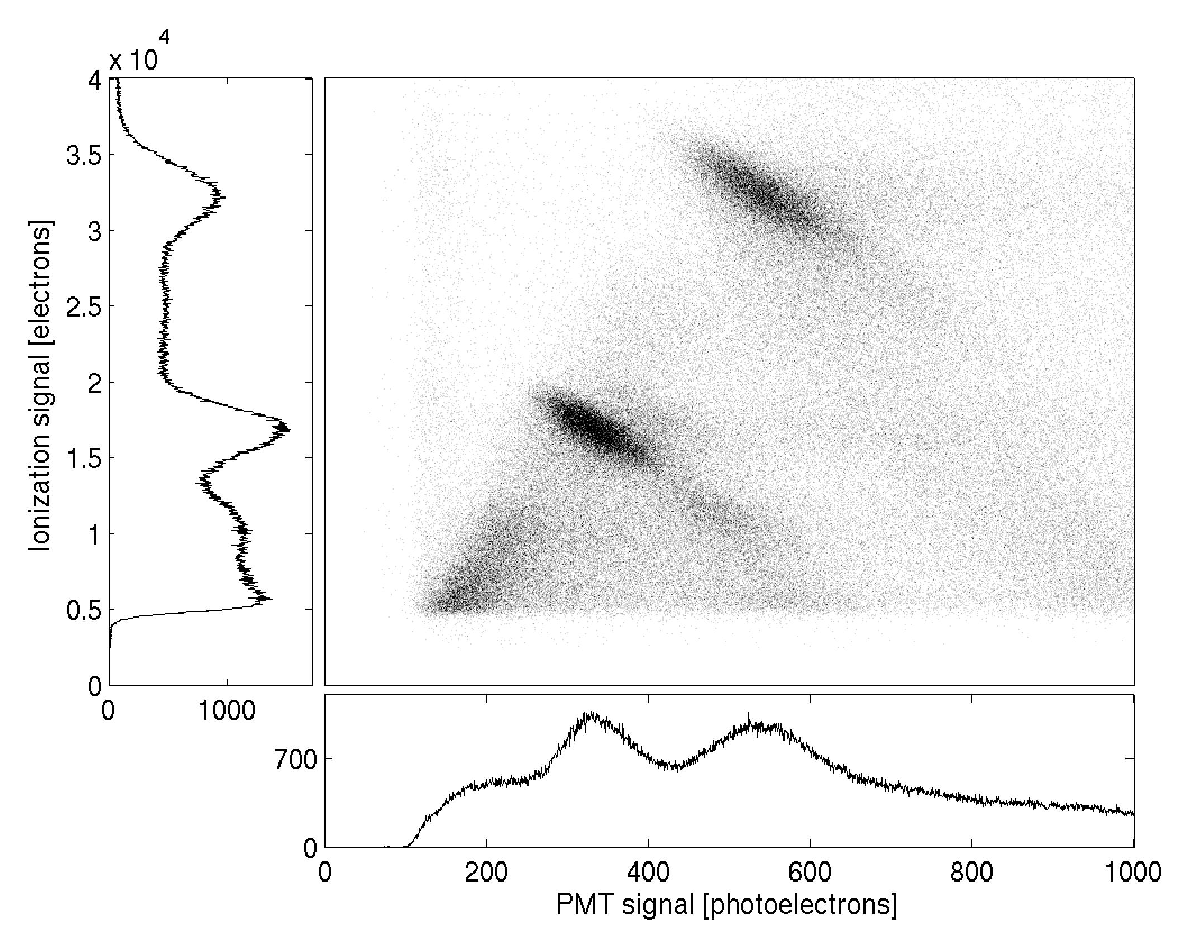
\includegraphics[keepaspectratio=true,width=\textwidth]{4kV_correl1.eps}
\end{center}
\renewcommand{\baselinestretch}{1}
\small\normalsize
\begin{quote}
\caption{A two-dimensional energy spectrum of scintillation and ionization from a testbed liquid xenon experiment under an electric field of $4$ kV/cm.  The spectrum is from a $^{207}$Bi source.  Figure reproduced from~\cite{PhysRevB.68.054201}.}
\label{fig:AnticorrelationInXenon}
\end{quote}
\end{figure}
\renewcommand{\baselinestretch}{2}
\small\normalsize

Energy deposits in xenon can be measured primarily in two ways: optical photons are emitted from the excitation and de-excitation of atomic electrons of xenon, and xenon atoms are ionized to produce free electrons.  It is well-known~\cite{PhysRevB.68.054201} that liquid noble element calorimeters show significant fluctuations in their separate production of scintillation photons and free electrons, but that these separate quantities are strongly anticorrelated.  As a result, is it possible to achieve far better energy resolution if both light and charge are independently measured than if only one is detected; figure~\ref{fig:AnticorrelationInXenon} illustrates this phenomenon in a testbed liquid xenon experiment, where it is apparent that using light and charge simultaneously lets us observe narrower gamma lines than either individually.

\begin{figure}
\begin{center}
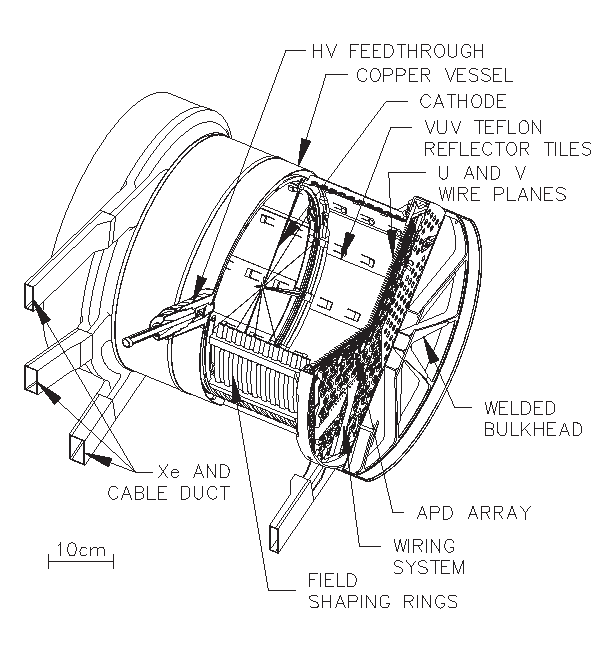
\includegraphics[keepaspectratio=true,width=\textwidth]{TPCSchematic.eps}
\end{center}
\renewcommand{\baselinestretch}{1}
\small\normalsize
\begin{quote}
\caption{Schematic of the inner EXO-200 TPC.  Figure reproduced from~\cite{detectorPartI}.}
\label{fig:TPCSchematic}
\end{quote}
\end{figure}
\renewcommand{\baselinestretch}{2}
\small\normalsize

Scintillation will be produced from energy deposits in liquid xenon in all cases;~\cite{Thesis_EDahl} however, to observe free electrons we must exert an electric field on the xenon which drifts the electrons onto a collection anode.  The EXO-200 detector is shaped as a cylinder, and the required electric field is produced by placing a cathode grid in the center of that cylinder and anode wires along each of the two endcaps of the detector; such a detector is called a time projection chamber, or TPC.  The EXO TPC is shown in figure~\ref{fig:TPCSchematic}.  The light is collected by avalanche photo-diodes (see section~\ref{sec:DetectorReadout} for details) mounted on the endcaps behind the anode wires; the anode wires are thin, so the effect on light collection efficiency is minimal.

The cathode is maintained at a voltage of $8$ kV above the anode wire voltage.  Field shaping rings encircle the outside of the EXO cylinder to ensure that electric field lines are approximately parallel and the magnitude of the electric field is roughly constant in the bulk volume of xenon.  (Near the edges, non-uniformities in the electric field are believed to exist; these are a continuing topic of research.)  The cathode and anode wires are separated by roughly $20.4$ cm; after accounting for edge effects, we believe that the bulk volume of xenon has an electric field of roughly $374$ V/cm.

Electrons in liquid xenon drift at a velocity of $1.71$ mm/$\mu$s under an electric field of $375$ V/cm.  The maximum drift distance from the cathode to the anode is $198.4$ mm, resulting in a maximum electron drift time of roughly $116$ $\mu$s.  Free electrons are not absorbed by xenon -- as for other noble elements, xenon has a low electronegativity, so in a pure xenon detector electrons could drift unimpeded for the time necessary to reach the anode.  EXO-200 does have small quantities of electronegative impurities such as oxygen and methane; to minimize the concentration of these impurities, the xenon of EXO-200 is constantly circulated through a chemical purifier which extracts chemically active molecules and permits noble elements to pass through.~\cite{detectorPartI}

It is necessary to associate charge pulses with their corresponding scintillation pulses in spite of their time separation.  However, this is easily done provided the time between events is much longer than $116$ $\mu$s.  Thus, sources should be calibrated to produce a data rate in xenon no higher than roughly $1$ kHz.  By measuring the time difference between the observation of scintillation and the collection of charge, we can measure the position of the energy deposit along one dimension.  Our time resolution permits us to reconstruct this position coordinate with an accuracy of $0.42$ mm.~\cite{bb2nEXO2014}

\begin{figure}
\begin{center}
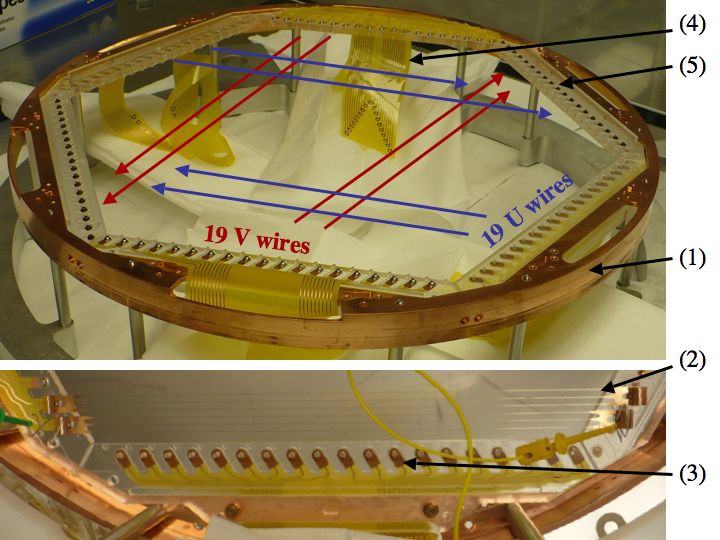
\includegraphics[keepaspectratio=true,width=\textwidth]{supportwithoutwires.png}
\end{center}
\renewcommand{\baselinestretch}{1}
\small\normalsize
\begin{quote}
\caption{Anode collection wires (u-wires) and induction wires (v-wires) from EXO-200.  (1) and (5) indicate the wire support frame; (2) indicates the wires themselves, constructed as gangs of three wires; (3) illustrates the attachment between wires and the support frame; (4) shows the return cables from the wires to the data acquisition system.  Figure reproduced from~\cite{detectorPartI}.}
\label{fig:UandVWiresCrossing}
\end{quote}
\end{figure}
\renewcommand{\baselinestretch}{2}
\small\normalsize

At the anode, there are two sets of parallel wire planes.  The first (closer to the cathode) parallel wire plane is called the ``v-wire'' plane, and the second plane is called the ``u-wire'' plane.  The voltages of the two wire planes are set so that no elecric field lines terminate on the v-wires, and all field lines instead penetrate through the v-wire plane and terminate on the u-wires.  When charge is deposited within the liquid xenon and drifts toward the anode, it induces a current on the v-wires as it passes by, and then produces a current on the u-wires as it is collected.

Figure~\ref{fig:UandVWiresCrossing} indicates the relative orientation of the u-wires and v-wires.  By detecting which (set of) wires observes a current pulse in both the u-wire and v-wire channels, it is possible to identify the two-dimensional location on the anode where the charge arrived.  Channels in each plane are $9$ mm wide; by taking advantage of signal sharing which sometimes occurs between u-wires and always occurs between v-wires, we are able to achieve position accuracy of $2.4$ mm perpendicular to the u-wires and $1.2$ mm perpendicular to the v-wires.~\cite{bb2nEXO2014}

Energy which appears to come from a single location is called a charge deposit ``cluster'' or ``site'', and events are classified according to the number of sites they produce (their ``multiplicity'') as either single-site or multi-site.  We will see in section~\ref{sec:DetectorActiveBackgroundRejection} that this is provides a powerful tool for background rejection.

This section has described how energy deposits in the liquid xenon are transformed into scintillation and charge, which are then observed by APDs and anode wires, respectively.  These observations are sufficient for us to reconstruct the positions and magnitudes of energy deposits in the liquid xenon.

\section{Backgrounds to \texorpdfstring{$\beta\beta 0\nu$}{Neutrinoless Double-Beta} Decay}\label{sec:DetectorBackgrounds}

$^{136}$Xe has a relatively high $Q$-value compared to most other $\beta\beta$ decays; in the neutrinoless mode the two emitted electrons will share $2456.7$ keV.~\cite{NewEXObb0nPaper_2014}  This means that the sensitivity of $T_{1/2}^{0\nu}$ to the mass of the neutrino is good in $^{136}$Xe, as was described in section~\ref{sec:NucPhysConstraintsFromBB0N}; it also means that energy spectrum around our $Q$-value will naturally be relatively free from most sources of background radiation.  This section will identify the types of background which can be expected to affect our $\beta\beta 0\nu$ search; subsequent sections will describe methods of mitigating those backgrounds.

It is common for alpha decays to have energies well in excess of our $Q$-value.  As a result, we might expect all alpha decays to be possible backgrounds to $\beta\beta 0\nu$.  However, alpha particles are stopped rapidly by even a small quantity of shielding, and as a result the only alpha decays which can be observed in the detector are those from sources which are dissolved into the xenon.  Radon is the only alpha-emitting noble element, and only $^{222}$Rn is sufficiently long-lived to diffuse into the xenon; as a result, we only expect $^{222}$Rn and its daughter products to contribute a significant quantity of alpha decays to the detector.

Cosmic rays produce high-energy muons; these are another source of high-energy backgrounds.  Muons will produce a streak of energy in the detector rather than discrete clusters; generally they will have sufficient energy to pass fully through the detector.  We can expect that such an event will look substantially different from a $\beta\beta 0\nu$ event, and generally will deposit substantially more energy than our $Q$-value as well.

More interesting are the associated by-products from the passage of such a high-energy particle, called spallation products.  Although high-energy muons can produce a range of fission products, the most significant spallation product of muons will be neutrons which can diffuse into the detector and activate materials there.  $^{134}$Xe and $^{136}$Xe are both present in significant quantities in the TPC, and by activation can be converted into the radioactive isotopes $^{135}$Xe and $^{137}$Xe respectively.  $^{135}$Xe has too little energy to be a background to $\beta\beta 0\nu$ decay, but $^{137}$Xe undergoes $\beta$ decay with a maximum energy of $4173$ keV.  We will see that indeed $^{137}$Xe is a significant source of background in our detector.~\cite{NewEXObb0nPaper_2014}~\cite{NeutronCaptureGammas}

Some sources of background are intrinsic to the $\beta\beta 0\nu$ search.  Any isotope which can undergo $\beta\beta 0\nu$ decay can also undergo $\beta\beta 2\nu$ decay, and the endpoint of the $\beta\beta 2\nu$ spectrum is necessarily at our $Q$-value.  The only means of reducing background from $\beta\beta 2\nu$ is to improve the energy resolution of the detector so that fewer such decays can mimic $\beta\beta 0\nu$ decay.  Fortunately with the energy resolution exhibited by the EXO-200 detector, $\beta\beta 2\nu$ is subdominant to other backgrounds by many orders of magnitude.~\cite{NewEXObb0nPaper_2014}

Similarly, it is hypothetically possible for neutrino absorption to stimulate a $\beta\beta 2\nu$ decay by the reaction
\begin{equation}
2d + \nu_e \rightarrow 2u + 2e^- + \bar{\nu}_e
\end{equation}
which is obtained from the $\beta\beta 2\nu$ reaction by taking one neutrino from product to reactant in equation~\ref{eqn:bb2n_decay_reaction}.  The observable spectrum is similar to the standard $\beta\beta 2\nu$ spectrum, but with the endpoint shifted upward by the energy of the absorbed neutrino.  The cross-section for this reaction is excpected to be well below the cross-section for standard $\beta\beta 2\nu$, so this will be a negligible background well beyond the current generation of $\beta\beta$ detectors.

A gamma background which is particularly detrimental to EXO-200 comes from $^{214}$Bi, a member of the radium decay chain.  $^{214}$Bi emits a gamma particle at $2448$ keV, which with our energy resolution is indistinguishable from our $Q$-value.  It will occur as a daughter product of $^{226}$Ra, which has a half-life of $1600$ years and generally will be supported by $^{230}$Th ($75,000$ years), $^{234}$U ($250,000$ years), and ultimately by $^{238}$U ($4.5 \cdot 10^9$ years) which has a primordial abundance in the Earth's crust and most natural materials.~\cite{ENSDF}

Most other backgrounds to $\beta\beta 0\nu$ will be gamma decays from $^{208}$Tl, a member of the thorium decay chain.  $^{208}$Tl emits a gamma particle at $2614.5$ keV; with our $Q$-value of $2456.7$ keV, the two energies are separated by $157.8$ keV.~\cite{ENSDF}  The energy resolution (in $\sigma/\text{mean}$) of EXO-200 has typically been $1.5-2\%$ at these energies,~\cite{NewEXObb0nPaper_2014} meaning that separation between the central values of the gamma lines will be $3-4\sigma$.  The thorium decay chain is supported by $^{232}$Th, which has a half-life of $14$ billion years and has a significant abundance in most natural materials; we may expect it to contribute a significant fraction of our radioactive backgrounds, and as a result we may expect that some events from the $2615$ keV $^{208}$Tl line will leak across those $3-4\sigma$ and act as backgrounds.  Keeping our energy resolution at or below $1.5\%$ may be of significant interest in reducing contamination from this gamma line.

The compton edge is a well-known feature of gamma decay spectra; it originates from gammas which enter a calorimeter, scatter once, and escape from the detector.  The maximum energy which a gamma of incident energy $E_{inc}$ can deposit in a single compton scatter is:~\cite{Compton}
\begin{equation}
E_{dep} = \frac{2E_{inc}^2}{m_e c^2 + 2E_{inc}}.
\end{equation}
When the incident gamma has an energy of $2615$ keV, the compton edge will lie at $2382$ keV, or only $74.5$ keV below our $Q$-value.  Using the same estimate that our energy resolution is around $1.5-2\sigma$ at these energies, this separation is only around $1.5-2\sigma$.  It is clear that improving our energy resolution may have a strong impact on background contamination by improving separation from the compton edge of the $^{208}$Tl as well as its full deposit line.

We have here identified some of the primary backgrounds which can be expected in the EXO-200 detector, noting particularly those which can be significantly reduced through improvements to the energy resolution.  The following sections will identify some of the mechanisms used to further minimize these backgrounds.

\section{Passive Background Rejection}\label{sec:DetectorPassiveBackgroundRejection}

When we describe the methods by which backgrounds to $\beta\beta 0\nu$ are reduced, we can distinguish between two classes: passive methods in which backgrounds are reduced by reducing the amount of background reaching the xenon in the first place, and active methods in which backgrounds are observed by the detector but discriminated from $\beta\beta$ signal based on identifying characteristics.  In this section, passive methods will be described; section~\ref{sec:DetectorActiveBackgroundRejection} will describe the active methods of background rejection.

\begin{figure}
\begin{center}
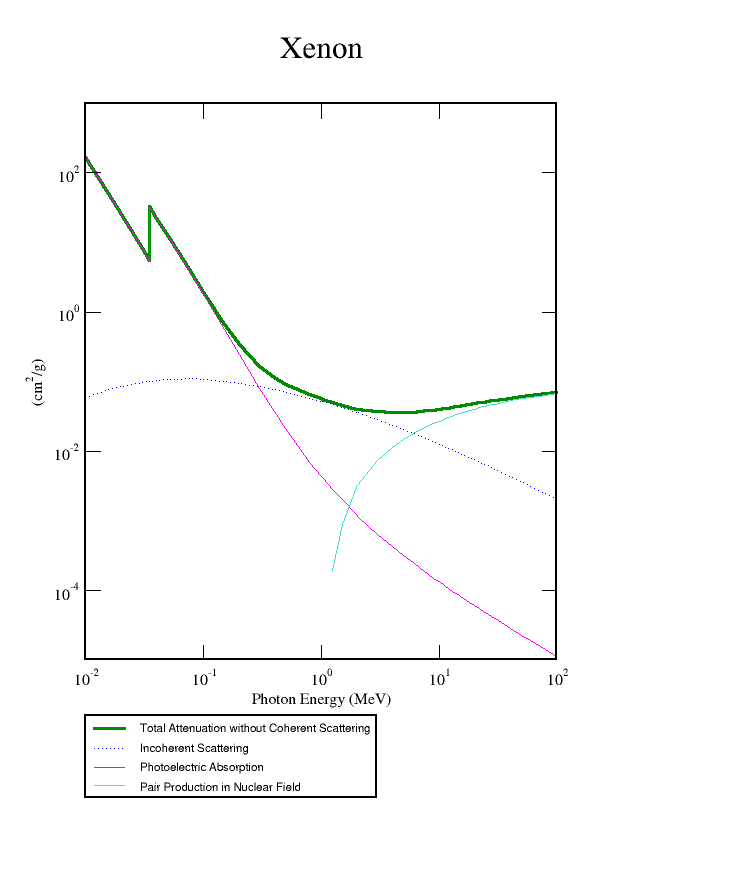
\includegraphics[keepaspectratio=true,width=\textwidth]{XrayAttenuationXenon.png}
\end{center}
\renewcommand{\baselinestretch}{1}
\small\normalsize
\begin{quote}
\caption{X-ray attenuation lengths in xenon.  Compton (incoherent) scattering, pair production, and photoelectric absorption are shown, along with their combined attenuation length; coherent (Rayleigh) scattering is omitted because it produces no observable energy deposit.  The vertical axis, in $\text{cm}^2/\text{g}$, can be multiplied by the density of the xenon to derive an attenuation factor per unit length.  Figure produced by~\cite{XcomXenonAttenuation}.}
\label{fig:XrayAttenuationXenon}
\end{quote}
\end{figure}
\renewcommand{\baselinestretch}{2}
\small\normalsize

The simplest and most immediate method of reducing the presence of backgrounds is by exploiting the self-shielding properties of xenon.  The xenon itself is extremely pure due to the easy of chemical purification; as a result most backgrounds will be external to the xenon.  Since external gammas are attenuated by dense materials such as liquid xenon, we can expect that the xenon near the center of the detector will be exposed to less background than the xenon near the TPC walls.  This is one of the primary advantages of xenon as a source: it is easy to construct a large monolithic detector, maximizing the quantity of xenon which is shielded from the walls.

Figure~\ref{fig:XrayAttenuationXenon} shows the attenuation lengths of gammas at a range of energies in xenon.  Photoabsorption and pair production both convert the gamma entirely into short-ranged electron and positron carriers; compton (incoherent) scattering results in only some deposited energy, with the rest remaining in the gamma which will rebound and continue on its path.  Liquid xenon has a density around $3$ g/cm$^3$, which means that the minimum attenuation factor is roughly $0.1/\text{cm}$ at energies around $4$ MeV.  Unfortunately, this is the same order of magnitude as our $Q$-value at $2456.7$ keV, which means that at the energy of interest to us self-shielding is minimally effective.  Nevertheless, there will still be some reduction in backgrounds deeper in the interior of the xenon, and lower-energy gammas will be attenuated more effectively.~\cite{XcomXenonAttenuation}

To reduce the quantity of background around the detector, all materials near the xenon were carefully screened for radioactive contamination.  Backgrounds from $^{40}$K, $^{232}$Th, and $^{238}$U were cataloged for all materials which have unshielded line-of-site access to the detector system.  Requirements for $^{238}$U were particularly stringent because its daughter products include the $^{214}$Bi background which cannot be resolved from $\beta\beta 0\nu$ decay.  For the copper of the TPC vessel and the lead shielding around the detector apparatus, samples from a range of companies and mines were tested to locate an optimal choice of material source.  For the wires which were placed into the TPC, a range of manufacturing methods were tested; improvements to a photo-etching scheme were identified which led to a reduction in background from these materials.  This thorough material screening research is one of the distinctive processes which has enabled EXO-200 to fully reach its background targets.  Details of the quantification of and constraints on material radioactivity can be found in~\cite{MaterialsCatalog}.

Beyond selecting extremely clean materials, it is possible to reduce backgrounds by minimizing the mass of these external materials.  Most notably, EXO-200 is constructed with a copper TPC which in most places is only $1.37$ mm thick; to maintain structural integrity, supporting structures are welded to the TPC where needed, and it was possible to keep the total mass of copper below $30$ kg.~\cite{detectorPartI}

Some materials were dispensed with entirely.  Typically, silicon APDs are encapsulated with ceramic to isolate them from water contamination and provide electrical insulation.  However, this ceramic material would have contributed backgrounds.  Instead, the APDs were delivered ``bare,'' without any encapsulation, and protected from water by storing them in a dry-nitrogen container.  Liquid xenon itself serves as an excellent electrical insulator, ensuring the APDs would function properly during detector operations.~\cite{EXOLAAPD}

\begin{figure}
\begin{center}
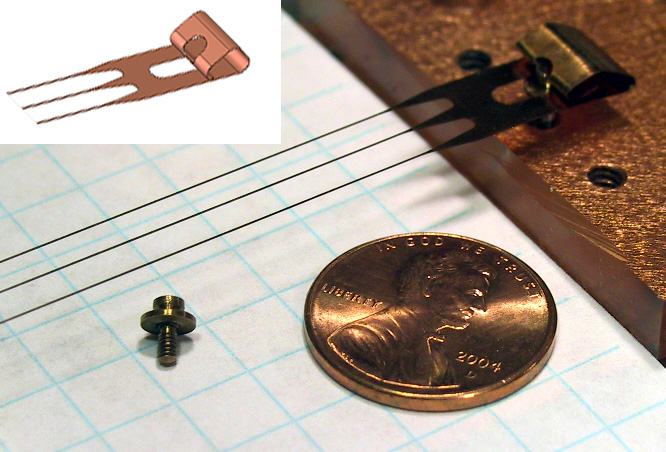
\includegraphics[keepaspectratio=true,width=\textwidth]{triplet.jpg}
\end{center}
\renewcommand{\baselinestretch}{1}
\small\normalsize
\begin{quote}
\caption{Wire triplet, read as one channel.  Figure from~\cite{detectorPartI}.}
\label{fig:WireTriplet}
\end{quote}
\end{figure}
\renewcommand{\baselinestretch}{2}
\small\normalsize

\begin{figure}
\begin{center}
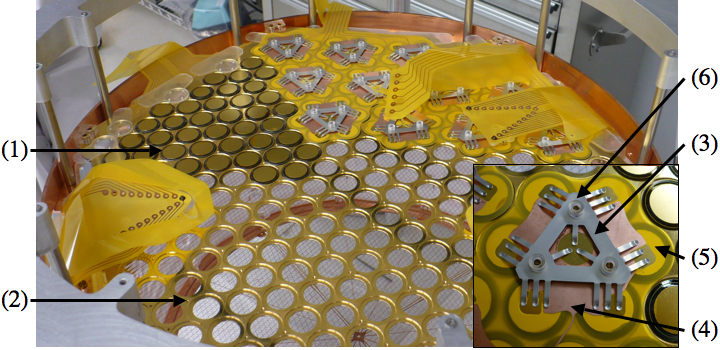
\includegraphics[keepaspectratio=true,width=\textwidth]{PlatterWGO7.png}
\end{center}
\renewcommand{\baselinestretch}{1}
\small\normalsize
\begin{quote}
\caption{APDs ganged together (bottom right).  Wiring to the front-end electronics are visible as yellow ``tape.''  Figure from~\cite{detectorPartI}.}
\label{fig:APDgang}
\end{quote}
\end{figure}
\renewcommand{\baselinestretch}{2}
\small\normalsize

Another example of material avoidance comes from the cabling from wires and APDs to the electrical amplifiers and digitizers.  These electronics contain many high-background plastics and other complex materials, so they were placed outside the lead shielding rather than placing them close to the TPC.  Wires connect the sensors in the TPC to these electronics; ordinarily such long wires would need to be shielded by coaxial cabling to minimize cross-talk noise.  However, the coaxial cabling was expected to contribute a high quantity of radioactive background, and was omitted; instead wires are partially shielded by surrounding them with inactive wires which reduce cross-talk noise.  Furthermore, the total number of wires needed was reduced by ganging together triplets of u- and v-wires and groups of six or seven APDs into single channels; this reduced the fineness of event information available in analysis, but reduced the quantity and complexity of material placed near the detector.  See the wire gangs in figure~\ref{fig:WireTriplet}; APD gangs and wiring to external electronics are visible in figure~\ref{fig:APDgang}.~\cite{detectorPartI}

\begin{figure}
\begin{center}
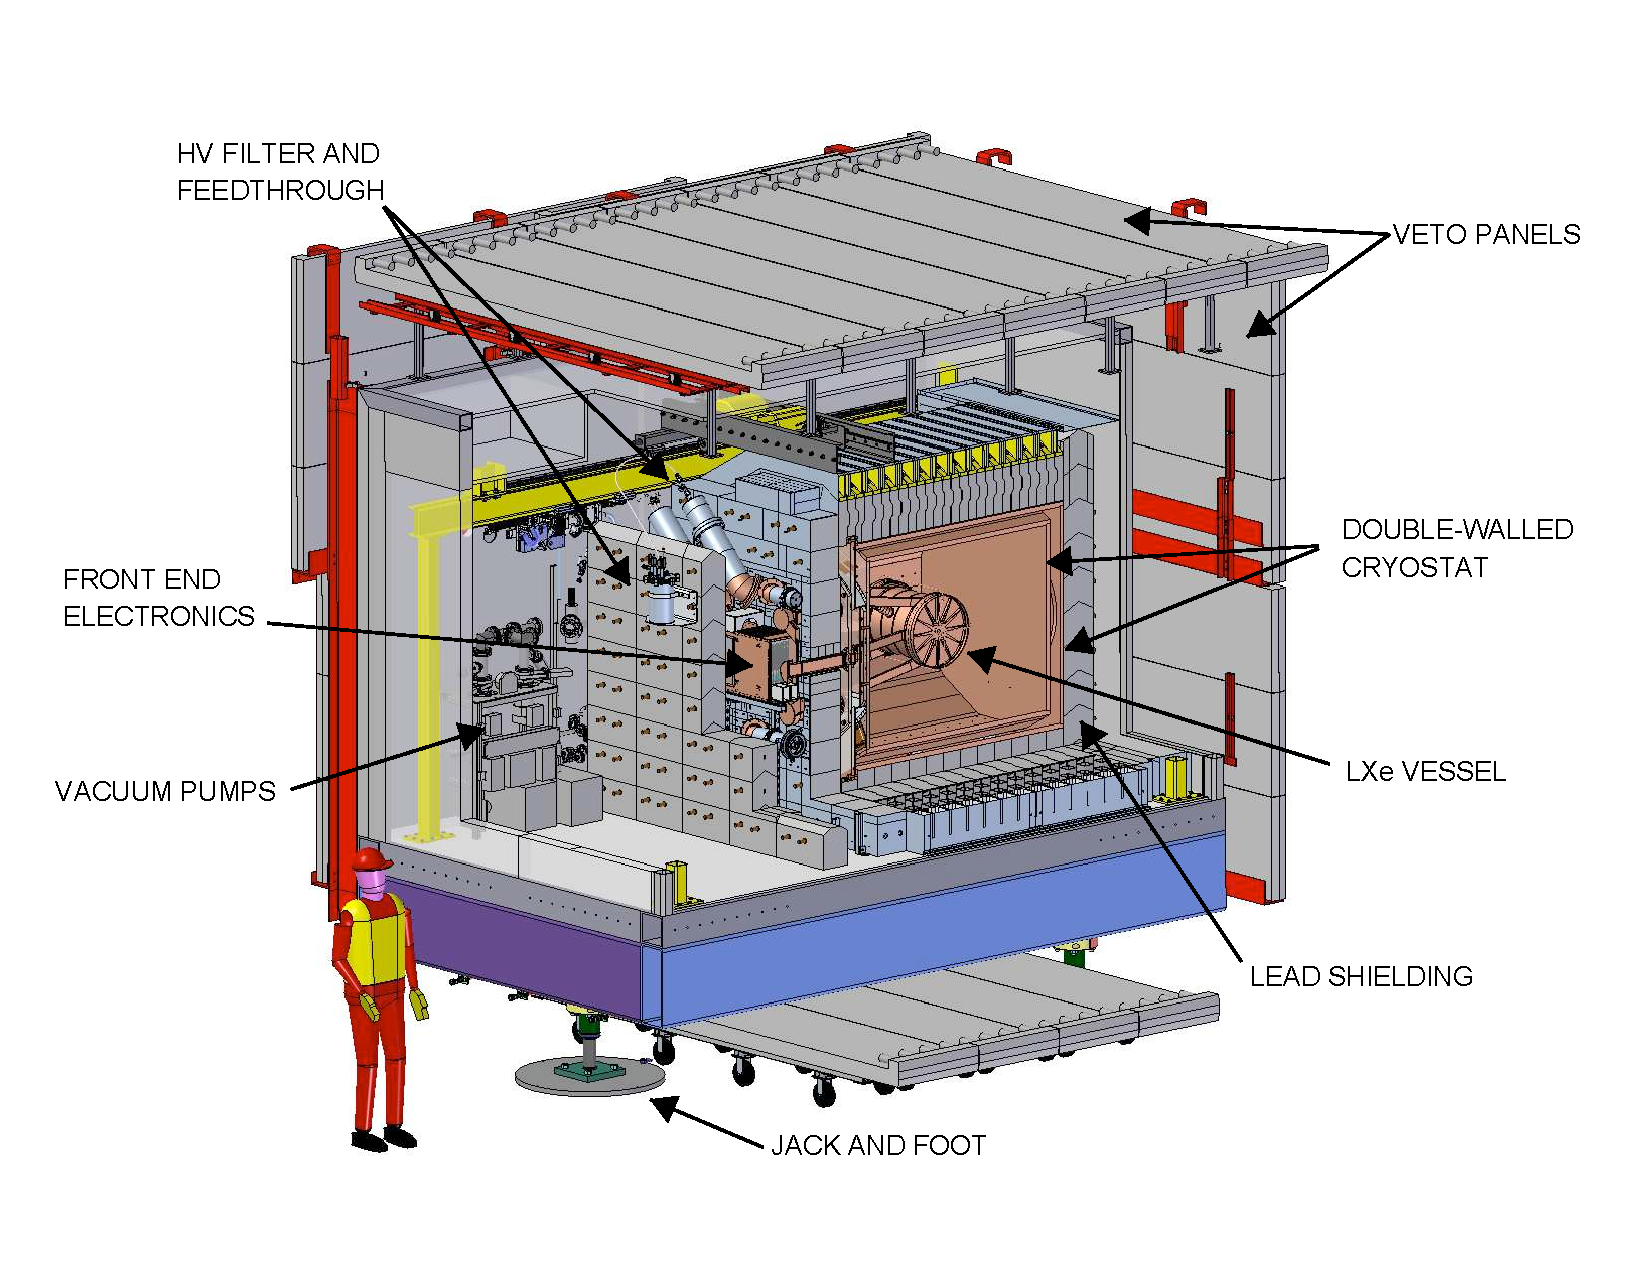
\includegraphics[keepaspectratio=true,width=\textwidth]{cleanroom.pdf}
\end{center}
\renewcommand{\baselinestretch}{1}
\small\normalsize
\begin{quote}
\caption{A cutaway schematic image of the TPC and surrounding materials in the cleanroom.  HFE-7000 refrigerant is contained between the cryostat and the LXe vessel.  Figure from~\cite{detectorPartI}.}
\label{fig:CleanRoomCutaway}
\end{quote}
\end{figure}
\renewcommand{\baselinestretch}{2}
\small\normalsize

We can imagine the TPC being shielded by nested layers of clean material designed to prevent backgrounds from reaching the xenon.  In the innermost layer, HFE-7000 refrigerant (see figure~\ref{fig:CleanRoomCutaway}) is used to maintain the detector at liquid xenon temperatures and maintain similar pressures inside and outside of the copper vessel walls.  However, the HFE has a significant quantity of hydrogen, which makes it an excellent stopping agent for thermal neutrons.  The refrigerant layer is more than $50$ cm thick, so most neutron products of muons have time to thermalize and absorb onto hydrogen before reaching the TPC and producing $^{137}$Xe.~\cite{detectorPartI}

The following layer of shielding is lead, shown in figure~\ref{fig:CleanRoomCutaway}.  This is a common approach for low-background experiments due to the high density of lead, which enables it to stop gammas in a short distance.  Lead bricks surround the detector on all sides; the bricks were designed with an interlocking shape to ensure no seams between bricks left a line-of-sight path from external sources into the TPC.  In the front of the detector, where plumbing must enter and exit the detector through the first lead wall, a second lead wall is assembled with the purpose of blocking any line-of-sight paths into the TPC through the plumbing gaps of the first wall.~\cite{detectorPartI}

\begin{figure}
\begin{center}
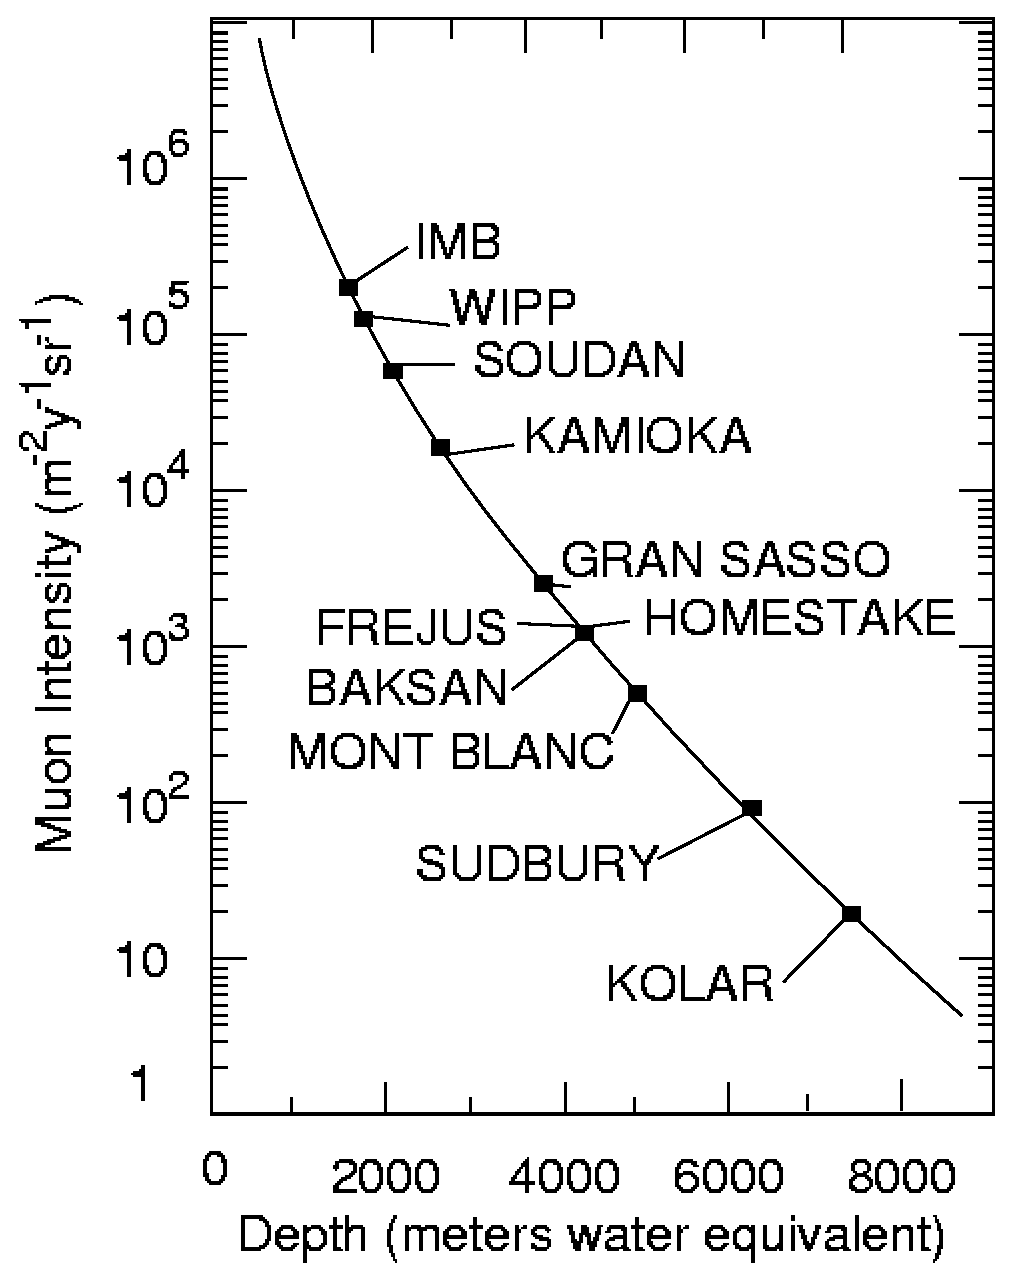
\includegraphics[keepaspectratio=true,width=\textwidth]{muonflux.eps}
\end{center}
\renewcommand{\baselinestretch}{1}
\small\normalsize
\begin{quote}
\caption{Muon flux as a function of depth, in meters water equivalent.  The WIPP site is indicated in relation to other underground science facilities.  Figure from~\cite{Esch2005516}.}
\label{fig:MuonFluxVsDepth}
\end{quote}
\end{figure}
\renewcommand{\baselinestretch}{2}
\small\normalsize

Outside of the lead shielding, restrictions on materials are less stringent; however, control over the presence of materials is still desired.  The entire apparatus is contained inside a class-1000 clean room facility.  Entire facility is located in the Waste Isolation Pilot Plant (WIPP) facility, a DOE-owned waste repository located in a salt mine in Carlsbad, NM.  The overburden of the facility is $1585$ m water-equivalent, leading to a significant reduction in muon rate compared to the rate observed on the Earth's surface.  Figure~\ref{fig:MuonFluxVsDepth} demonstrated the reduction in muon flux due to depth at the WIPP site and a selection of other underground science facilities.

These passive approaches have all been demonstrated to reduce the rate of backgrounds depositing energy in the liquid xenon.  The following section will describe an active set of background-rejection approaches.

\section{Active Background Rejection}\label{sec:DetectorActiveBackgroundRejection}

This section will describe the ``active'' forms of background reduction employed by the EXO-200 detector, in which events are observed but discriminated from $\beta\beta$ events based on their characteristics.  We neglect the energy resolution as a background rejection tool here, since section~\ref{sec:DetectorBackgrounds} has already described how the impact of certain backgrounds may be reduced by improvement to the energy resolution.

A number of cosmogenic backgrounds have been described: neutrons and fission products can be produced from muons penetating down to the depth of the WIPP facility.  To reject many of these events, it is sufficient to detect the passage of a muon anywhere near the detector.  This is accomplished by means of a set of veto panels surrounding the cleanroom on four of six sides.  Muons are detected by coincident panel hits on opposite sides of the detector, with $(96.0 \pm 0.5)\%$ efficiency for detecting muons which traverse the TPC.~\cite{detectorPartI}  Further reduction in the impact of muon-induced backgrounds is achieved by searching for muon tracks observed within the TPC itself, and also by applying a one-second coincident event cut as a catch-all for spallation products of muons which may decay multiple times in rapid succession.

Alpha decays within the xenon were identified as another possible source of high-energy backgrounds.  However, it is possible to discriminate alpha decays from beta and gamma decays based on the properties of their energy measurement.  Alphas produce a far more dense energy deposit in liquid xenon than betas and gammas; the dense collection of free electrons and ionized xenon has a higher rate of recombination than is observed with betas and gammas, which translates into a higher ratio of scintillation to ionization for alphas than for betas and gammas.  This feature can be used to eliminate nearly all alpha background.

Discriminating between gamma, beta, and double-beta decays is more difficult.  Gammas generally deposit their energy by ionizing atomic electrons of xenon, so in this way their behavior may closely mimic that of betas.  However, most gammas within our energy window (and particularly gammas near our $Q$-value) will be attenuated by compton (incoherent) scattering, as can be seen in figure~\ref{fig:XrayAttenuationXenon}.  By this process the gamma will deposit energy in more than one discrete location, which beta and double-beta decay will not do.  We are generally able to resolve the positions of these energy deposits and classify the event as multi-site; more than half of external gamma backgrounds are classified as multi-site, whereas the fraction of $\beta\beta$ events classified as multi-site is only $5\%$.~\cite{bb2nEXO2014}

These are some of the basic techniques employed to reduce backgrounds in offline analysis, and the detector has been designed with the goal of facilitating their application.  Although the passive methods of background reduction cannot be improved once construction of the detector is complete, it may be hoped that these active methods may be improved or extended through further analysis.  These improvements could have the potential to reduce backgrounds in data which has already been collected, making them a particularly attractive target now that EXO-200 has collected a significant dataset.

\section{Pulse Amplification and Waveform Readout}\label{sec:DetectorReadout}

After an APD or wire collects a signal, how is it converted into a waveform on disk?  This section will provide a brief overview of the EXO electronics and waveform readout.  Particular attention will be paid to subsystems which are relevant to the denoising algorithm described in chapter~\ref{ch:DenoisingTheory}, including the APDs and front-end electronics.

\begin{figure}
\begin{center}
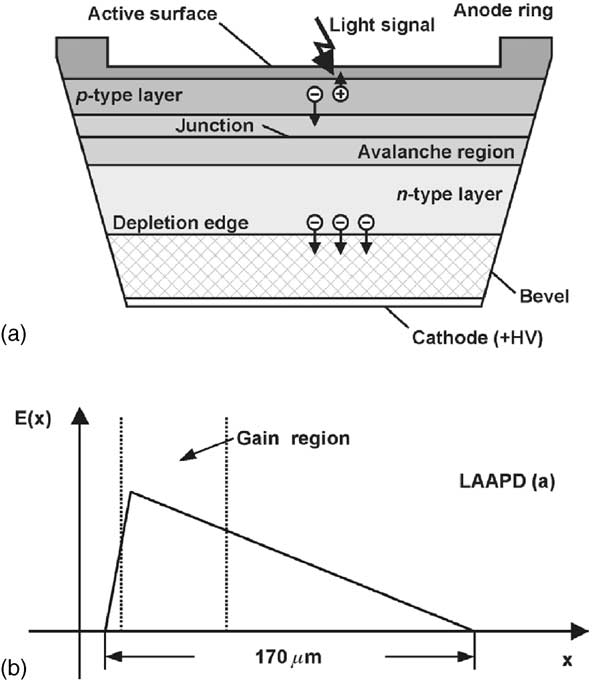
\includegraphics[keepaspectratio=true,width=\textwidth]{APDCrossSection.png}
\end{center}
\renewcommand{\baselinestretch}{1}
\small\normalsize
\begin{quote}
\caption{A cross-sectional schematic of an APD is shown in (a).  The electric field as a function of depth is shown in (b).  Figure from~\cite{Moszynski2002504}.}
\label{fig:APDCrossSection}
\end{quote}
\end{figure}
\renewcommand{\baselinestretch}{2}
\small\normalsize

The APDs are constructed from a silicon semiconductor which is doped and biased so that:~\cite{Moszynski2002504}
\begin{enumerate}
\item Photons arriving at the active surface of the APD can deposit their energy by generating an electron-hole pair in the silicon semiconductor.
\item The electron-hole pair is drifted apart by an electric field.  Here the electric field is low and the silicon is doped to be of p-type (electron-poor), ensuring a similar number of electron-hole pairs are produced by all photons before any amplification can occur.
\item The electron enters a high-field n-type (electron-rich) region of silicon, and liberates additional electron-hole pairs in an avalanche effect.
\item Electrons reach another p-type region of silicon, and then are collected on a cathode as an output current pulse.
\end{enumerate}
These phases of the APD are illustrated in figure~\ref{fig:APDCrossSection}.

EXO-200 had $851$ APDs specially made with pure aluminum and no casing; from those, $468$ were selected for use based on their excellent noise and gain properties.~\cite{EXOLAAPD}  For each APD, the relative quantum efficiency for electron-hole production and the bias voltage needed to ensure the product of gain and quantum efficiency equals one hundred were both measured.  APDs were assigned to gangs and pies so that their products of gain and quantum efficiency could be set to one hundred as uniformly as possible.~\cite{APDMeasurementAndGanging}  It is impossible to make the gain of all APDs perfectly uniform because of limitations in the configurability of the APD bias voltages in EXO-200.~\cite{detectorPartI}  We note that the current operating conditions of EXO-200 establish a higher operating gain of around $200-300$; this may have the side effect of making the product of gain and quantum efficiency less uniform in each APD gang.

The means by which wires deliver charge is somewhat simpler than for APDs.  In the u-wires, charge is collected and delivered directly to the electronics as current.  In the v-wires, no net charge is delivered, but transient currents are induced in such a way that the v-wire remains at a constant voltage; these transient currents produce a pulse with a different shape than the u-wire pulses, such that the integral (before shaping) is zero.  We note that the pulse shape depends on the path of electrons in the xenon -- both sets of wires deliver a current signal which is induced from approaching charge before the charge deposits on the u-wires, and the path of the electrons can affect the timing of that induced current.  Furthermore, the pulse magnitude will depend on the point of origin of the electrons because at that location positively-charged ions will remain long after the electrons have been collected, and the ions will hold a net charge on the u- and v-wires which is released only on much longer timescales than we can observe in our waveforms.  (Ions, being much more massive than electrons, drift much more slowly through liquid xenon.)~\cite{EnergyDocumentRun2a}~\cite{MCDocumentRun2a}

The front-end electronics, located between the two lead walls in front of the detector, consist of four stages:~\cite{detectorPartI}~\cite{ReconstructionDocument}
\begin{enumerate}
\item A transimpedance amplifier which converts the current signals from the detector to voltage signals.  This stage applies amplification and a differentiator with a long time constant (roughly $60\mu$s for wires and $300\mu$s for APDs).
\item Two differentiators and two integrators, to improve signal-to-noise ratio for real-time triggering.  For the u-wires, each integrator has a time constant of $1.5\mu$s and each differentiator has a time constant of $40\mu$s; for the APDs and v-wires, each integrator has a time constant of $3\mu$s and each differentiator has a time constant of $10\mu$s.  Some signal amplification is applied at this stage as well.
\item An analog-to-digital converter (ADC) converts voltage pulses into $12$-bit digital waveforms.  The full $12$-bit scale is equivalent to $2.5$V.  Digitization is performed at a rate of $1$MHz.
\item A triggering module reads the digitized waveforms, and issues a trigger to the data acquisition (DAQ) when signals exceed programmable thresholds.  The triggering module can also accept external requests for a ``solicited'' trigger.
\end{enumerate}
In most cases, when a trigger is issued, the DAQ will write out $2048$ samples (just over $2$ms) from all waveforms, centered on the first sample responsible for the trigger.  In cases where the data rate is high, waveforms can be truncated to a length less than $2048$ samples.

\section{Calibration Systems}\label{sec:DetectorCalibration}

Energy resolution has been discussed as a general feature of the detector which can have a significant impact on the reduction of backgrounds.   A significant factor in the resolution is the quality of the detector's absolute energy calibration.  This is particularly important because of the long lifetime of the experiment.  If the calibration of the detector drifts over time, this will be perceived in the cumulative low-background spectrum as a smearing out of energy peaks, worsening the effective resolution.  This section will describe some of the techniques used to produce an accurate time-dependent calibration for the detector.

\begin{figure}
\begin{center}
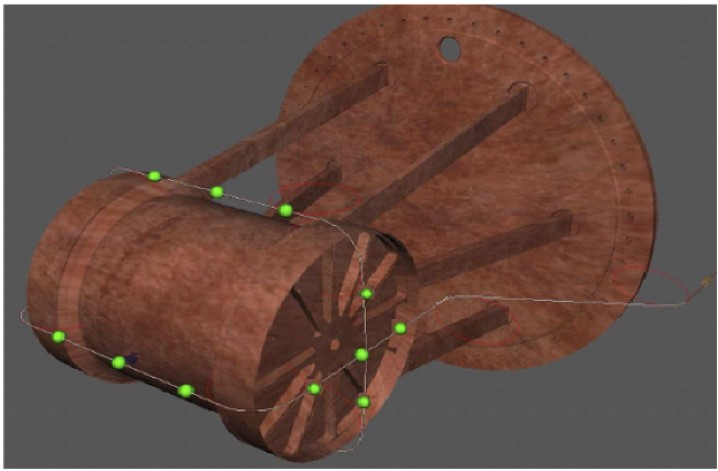
\includegraphics[keepaspectratio=true,width=\textwidth]{calibration_tube.jpg}
\end{center}
\renewcommand{\baselinestretch}{1}
\small\normalsize
\begin{quote}
\caption{A guide tube permits gamma sources to be inserted to known locations near the TPC.  Green dots indicate a few of the locations where the source may conventionally be placed.  Figure from~\cite{detectorPartI}.}
\label{fig:CalibrationGuideTube}
\end{quote}
\end{figure}
\renewcommand{\baselinestretch}{2}
\small\normalsize

The most critical type of calibration comes from external gamma sources.  The EXO experiment was constructed with a guide tube passing through the HFE refrigerant and wrapping loosely around the TPC, as shown in figure~\ref{fig:CalibrationGuideTube}.  Currently available to the experiment are sources containing $^{228}$Th (primary gamma line at $2615$ keV), $^{60}$Co (simultaneous emission of gammas at $1173$ and $1332$ keV), and $^{137}$Cs (gamma line at $662$ keV); additionally, a new $^{226}$Ra source became available in the summer of 2013 (numerous gammas, including $2448$ keV).  Together these sources allow us to observe the detector response to external gammas with known energies, permitting energy calibrations, energy resolution measurements, and verification of monte carlo simulations.

All of these sources have been used periodically (roughly every three months) in calibration campaigns intended to permit a full characterization of the detector response across a wide energy range at a particular moment.  Additionally, the $^{228}$Th source has been deployed regularly, typically three times every week for $2-3$ hours, for the entire history of the dataset.  The fullness of the $^{228}$Th source dataset, along with the benefit that it contains a relatively clean high-energy gamma line, make it a particularly convenient dataset to work with; it will play a prominent role in the generation of our lightmap described in chapter~\ref{ch:Lightmap}.

Other calibrations are also performed on the detector, and may in some instances supplement the information provided by the source data.  To perform direct calibrations of the APDs, one APD mount contains a light diffuser rather than an APD device; the diffuser can be illuminated by a laser through optical fibers.~\cite{detectorPartI}  The APDs can be calibrated by pulsing the laser while varying the voltages of the APDs to adjust their gain, and in this way it is possible to measure the gain of the APDs in situ.  A laser system was available at the beginning of the dataset used in this work; however, there were certain deficiencies to the laser system which made its data difficult to use, and as a result a new and more accurate laser system was commissioned in August 2012.  Laser data in some form has been collected roughly once per week for much of the time containing this dataset.  Composing the laser data into a coherent history of the APD gains is an ongoing project, but it has been possible to use APD gain information from specific moments to inform the APD noise model described in section~\ref{sec:DescriptionOfPhotonNoise}.

Just as it is possible and desirable to learn the gain of the APDs separately from other components using laser runs, it is also desirable to learn the gain of the electronics amplifiers separately from other detector function.  This is accomplished using ``internal calibrations:'' simultaneously with software triggers solicited by the data acquisition, a switched capacitor injects charge into the input of the electronics cards of individual or groups of channels.~\cite{EXOElectronicsFunctionalSpecification}  The resulting waveform is then read normally, and the size of the output pulse reflects the gain of the electronics.  This system is employed approximately daily on all channels; it provides an excellent measure of relative changes in the electronics gains over time.  However, the absolute gains cannot be extracted accurately from this data, and must be obtained by other means.

To measure the absolute gains of the electronics, the front-end cards must be physically removed from their enclosures; when this is done, it is possible to use a more accurately calibrated capacitor to make an absolute gain measurement in the same style as the internal calibrations.  These ``external calibrations'' can be performed in two flavors: manual, in which a capacitor calibrated to $1\%$ is used to inject charge, and automatic, in which the calibration is automatically performed at a much faster rate but accuracy is limited to $2-3\%$.  Due to the inconvenience of removing electronics cards from their enclosures, this process has only been performed once in February 2011.  Both styles of external calibration were performed on the u-wire channels.  Less demanding needs for resolution on the v-wires and APD channels were foreseen, so only the less accurate automatic calibration was performed on those channels.  The data from these runs has not been fully analyzed, but may be revived in future analysis to permit a better calibrations of the subsequent internal calibrations which were taken.~\cite{EnergyDocumentRun2a}

\section{Summary}

This chapter has described some of the key characteristics of the construction and operation of the EXO-200 detector.  Background reduction has been a theme throughout -- EXO-200 has employed both passive and active methods to reject background and improve its sensitivity to $\beta\beta 0\nu$ decay.  Energy resolution has also been described as a key element in background rejection because with sufficiently precise energy measurements, many backgrounds will no longer resemble $\beta\beta 0\nu$ decay.  Chapter~\ref{ch:DenoisingTheory} will begin our discussion of a new scheme to extract more accurate energy measurements from the APD channels, thereby improving our overall energy resolution and the sensitivity of the limit on the $\beta\beta 0\nu$ halflife we will be able to demonstrate.
